\subsection{definisi Operasi Pembagian}
operasi pembagian pada dasarnya adalah 
suatu proses pencarian tentang bilangan yang belum diketahui. Dikarena bentuk pembagian tersebut dapat di lihat dan kita pandang sebagai suatu bentuk operasi perkalian dengan salah satu faktor yang belum diketahui.

\subsection{SEJARAH}
Penemuan ini,  telah dirancang untuk memecahkan masalah dan objeknya adalah untuk menyediakan pembagi yang dapat melakukan pembagian dengan pembagi 
dan semua pembagi menjadi bilangan heksadesimal. Pembagi dari penemuan ini dibuat untuk menyelaraskan digit dari pembagi normalisasi normalisasi di muka 
dengan secara selektif menggunakan fungsi pergeseran dan fungsi pergeseran yang tepat yang dibangun pada pemilih, 
dan kemudian menentukan hasil pembagian heksadesimal dengan mengulangi proses dengan menentukan nomor kali.

Penemuan pertama pembagi yang terkait dengan penemuan ini dilengkapi dengan rangkaian normalisasi pertama untuk memasukkan data dari data floating point pembagi yang basisnya 16 dan menormalisasinya berdasarkan basis di atas, 
rangkaian normalisasi kedua untuk memasukkan data dari Pembagi adalah data floating point yang basisnya adalah 16 dan menormalisasinya berdasarkan basis di atas, rangkaian pembagi, 
dan pemilih untuk memasukkan data mantissa dari pembagi dari rangkaian normalisasi pertama, 
sisa data dari rangkaian pemisah dan sinyal siklus divisi yang menunjukkan siklus divisi, dan ketika sinyal siklus divisi menunjukkan siklus pertama,
melalui-keluaran data mantissa dari pembagian secara utuh, ketika sinyal siklus divisi menunjukkan siklus kedua dan data mantissa di bagi sama dengan atau lebih besar dari pada pembagi, 
menggeser data mantissa dari pembagi ke kanan dan mengeluarkannya, 
ketika sinyal siklus divisi menunjukkan siklus kedua dan mantiss data di bagi lebih kecil dari pada pembagi, 
menggeser data mantissa dari dividen ke kiri dan mengeluarkannya,
dan ketika sinyal siklus divisi menunjukkan siklus ketiga dan setelah ketiga, melalui pengeluaran data sisa utuh, 
dimana pembagi rangkaian menghitung data hasil bagi dan data sisa dari data yang dikeluarkan oleh pemilih dan data mantissa dari pembagi yang dikeluarkan oleh rangkaian normalisasi kedua.

Menurut penemuan kedua pembagi yang terkait dengan penemuan ini, shifter kiri di sirkuit pemisah biasanya digunakan di tempat shifter kiri yang diperlukan pada pemilih pada penemuan pertama oleh fakta bahwa selektor pembagi yang terkait dengan penemuan ini dibangun sedemikian rupa sehingga, 
ketika sinyal siklus divisi menunjukkan siklus pertama, ia mengeluarkan data mantissa dari dividen, ketika sinyal siklus divisi menunjukkan siklus kedua dan data mantissa dividen sama atau lebih besar dari pada pembagi , 
itu menggeser data mantissa dari dividen menjadi ketakutan dan mengeluarkannya, dan ketika sinyal siklus divisi menunjukkan siklus kedua dan data mantissa dividen lebih kecil dari pada pembagi atau ketika sinyal siklus divisi menunjukkan yang ketiga dan setelahnya siklus ketiga, itu data sisa sisa.

Dan menurut penemuan ketiga pembagi yang terkait dengan penemuan ini, pembagi dari penemuan pertama yang disebutkan di atas dikonstruksi sedemikian rupa sehingga melakukan pembagian bilangan desimal biner yang dicantumkan dan memperoleh data data yang dihasilkan dalam bentuk bilangan desimal biner yang terdaftar.

\subsection{Bilangan Biner}
Sejak pertama kali komputer digunakan, komputer beroperasi menggunakan bilangan biner, yaitu bilangan dengan basis 2 pada sistem bilangan. Semua kode program dan data pada komputer disimpan serta dimanipulasi dalam format biner yang merupakan kode-kode mesin komputer. Sehingga dari semua perhitungan tersebut yang dapat di olah menggunakan aritmatik, yaitu bilangan yang hanya memiliki dua kemungkinan adalah 0 dan 1, dan disebut juga sebagai bit (binary digit atau dalam arsitektur elektronik biasa disebut sebagai digital logic. Representasi bilangan biner bas dilihat disamping ini. Posisi sebuah angka akan menentukan berapa bobot nilainya. Posisi yang paling depan (kiri) sebuah bilangan memiliki nilai paling besar sehingga disebut sebagai MSB (Most Significant Bit), dan posisi paling belakang (kanan) sebuah bilangan memiliki nilai yang paling kecil sehinggal disebut sebagai LSB (Leased Significant Bit).

Contoh: reprentasi bilangan dengan basis biner:
\begin{equation}
101102 = 1*2^4 + 0*2^3+1*2^1+0*2^0=2210
\end{equation}

\subsection{Bilangan Heksadesimal}
Bilangan heksadesimal atau biasa disebut heksa saja, berbasis 16 memiliki nilai yang disimbolkan dengan 0, 1, 2, 3, 4, 5, 6, 7, 8, 9, a, b, c, d, e, f. Adanya bilanagn ini dikarenakan operasi bilangan biner untuk data yang lebih besar akan menjadi susah, hingga bilangan ini sering digunakan untuk menggambarkan memori computer atau intruksi. Setiap digit bilangan heksa mewakili 4 bit bilangan biner, dan 2 digit bilangan heksadesimal mewakili satu byte.
Sebagai contoh bilangan dari bilangan hexa 41 (2 nible), pada format ASCII ia mewakili karakter “A”, bilangan hexa 42 ia mewakili karakter “B”, dan segabainya.
\subsubsection{konversi}
Untuk mengkonversikannya ke dalam bilangan desimal, dapat kita gunakan formula berikut:
Bilangan heksadesimal H yang merupakan untaian dari digit hn hn-1… h2 h1 h0, jikalau dikonversikan menjadi bilangan desimal D, maka hasilnya seperti gambar ini\ref{rumus}
\begin{figure}[ht]
	\centerline{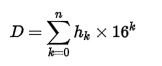
\includegraphics[width=1\textwidth]{figures/rumus.JPG}}
	\caption{rumus}
	\label{rumus}
	\end{figure}
Contohnya yaitu, bilangan heksa 10E yang akan di konversi ke dalam bilangan desimal:
\begin{itemize}
\item Digit digit 10E ini dapat menggantikan bilangan A sampai F (jika terdapat) dan menjadi bilangan desimal. Contohnya yaitu, 10E diubah menjadi barisan: 1,0,14 (E = 14 dalam basis 16)
\item Mengalikan dari tiap digit terhadap nilai tempatnya.
\end{itemize}
\begin{equation}
1 x 16^2 + 0 x 16^1 + 14 x 16^0
= 256 + 0 + 14
= 270
\end{equation}
Dengan demikian, bilangan 10E heksadesimal sama dengan bilangan desimal 270.


\subsection{contoh-contoh operasi bilangan}
Sebagai contoh apabila dalam perkalian 3 x 4 = k tentu k = 12 maka, dalam pembagian hal tersebut dapat dinyatakan,dengan bentuk 12 : 3 = n atau 12 : 4 = n
Dengan demikian 12 : 3 = n apabila dinyatakan dalam bentuk perkalian akan menjadi 12 = n x 3, sedangkan 12 : 4 = n menjadi bentuk perkalian menjadi 12 = n x 4. Untuk mencari nilai n dari bentuk 12 = n x 3, sama artinya dengan mencari jawab pertanyaan : bilangan manakah yang jika dikalikan dengan 3 akan menghasilkan 12 atau berapakah 12 : 3  Dua pertanyaan ini mungkin akan menghasilkan bilangan yang sama. Jadi apabila dalam pertanyaan yang pertama mendapatkan nilai 4, maka berarti pula nilai dari 12 : 3 = 4.
Pembagian bilangan bulat juga dapat dikelompokan menjadi empat, yaitu:
\begin{itemize}
\item Pembagian antara bilangan bulat positif dengan bilangan bulat positif 
\item Pembagian antara bilangan bulat positif dengan bilangan bulat negatif 
\item Pembagian antara bilangan bulat negatif dengan bilangan bulat positif 
\item Pembagian antara bilangan bulat negatif dengan bilangan bulat negatif Sama seperti pada operasi perkalian, pada operasi pembagian di kajian teoritis ini penulis hanya memaparkan operasi pembagian bilangan bulat positif dengan bilangan bulat positif
\end{itemize}

Untuk mendapatkan hasil pembagian bilangan bulat positif dengan bilangan bulat positif, yaitu dengan cara menggunakan pengurangan berulang sampai sisanya adalah nol. Hasil pembagian ditunjukkan dengan berapa banyak dikurangi dengan bilangan yang sama. Selanjutnya perhatikan contoh berikut ini: a. 10: 2= 10 - 2 - 2 - 2 - 2 - 2= 0 10 dikurangi 2 sebanyak 5 kali sampai sisanya 0. Artinya hasil dari 10 : 2 adalah 5. b. 24 : 4 = 24 - 4 - 4 - 4 - 4 - 4 - 4 = 0 24 dikurangi 4 sebanyak 6 kali sampai sisanya nol.
 Artinya hasilnya adalah 6. Operasi pembagian bilangan bulat positif dengan bilangan bulat positif dapat juga diperagakan dengan menggunakan garis bilangan. Untuk peragaan pada garis bilangan, kita ambil contoh pembagian berikut : 10 : 2. Untuk menentukan hasil pembagian tersebut dengan menggunakan garis bilangan adalah sebagai berikut. a. Siswa panah berkedudukan awal pada skala nol. b. Bilangan pembaginya adalah bilangan positif, maka ujung siswa panah akan menghadap ke arah bilangan positif. c. Siswa panah bergerak meloncat maju dengan setiap loncatan 2 skala, sebanyak 5 kali dan berhenti pada skala 10. d. Hasil pembagian 10 : 2 ditunjukkan dengan loncatan siswa panah sebanyak 5 loncatan maju yang berhenti pada skala 10. e. Jadi hasil dari 10 : 2 adalah 5.

\subsection{Kode Hex Representasi}
Misalkan delapan variable system minterms diekspresikan dalam biner dari (1).
Teknik ini cukup sulit untuk memvisualisasikan minterm dan juga berukuran besar. 
Hindari persamaan kesulitan ini (1) dapat digambarkan sebagai persamaan (2) dengan minterm kode desimal.
Persamaan (1) dapat diwakili dan direalisasikan sebagai 
(3) dengan menggunakan minterm kode gen heksadesimal, yang memerlukan sedikit operasi matematika berkenaan dengan teknik representasi yang digunakan pada (2).
Akhiran H digunakan sebagai indikasi minterm kode hex.
Demikian pula, maxterms juga memungkinkan untuk mewakili dengan bantuan heksadesimal kode maxterms. Teknik representasi yang diusulkan dengan mudah diperoleh dari tabel kebenaran dan dengan mudah ditemukan kembali dalam bentuk Biner bila diperlukan.
The hex codec minterms benar-benar memecah minterms menjadi pasangan empat variabel dari bit yang paling signifikan. 
Sepasang variabel empat terbobot terkecil yang kami sebut di sini Pasangan Sepenuhnya Signifikan dari variabel (LSP) berarti digit paling penting dari setiap minterms adalah LSP dan digit paling signifikan dari hex minterms adalah Most Significant Pair of variables (MSP). 
Tidak wajib bahwa MSP selalu memiliki sepasang empat variabel itu mungkin satu variabel juga, seperti kasus lima variabel sistem input. 

\subsection{konversi desimal menjadi biner melalui oktal}
Untuk bilangan bulat desimal yang mengandung beberapa digit, terbagi secara repeadly dengan 2 bisa menjadi proses yang panjang. 
Dalam kasus ini, biasanya lebih mudah untuk mengubah bilangan desimal menjadi bilangan biner melalui sistem bilangan oktal. 
Sistem ini memiliki radix 8, menggunakan angka 0, 1, 2, 3, 4, 5, 6 dan 7. 
Jumlah denatur yang setara dengan bilangan oktal 43178 adalah

\subsection{Digit nomor}
Digit nomor
Simbol seperti itu digunakan dalam sistem penomoran atau salah satu dari sepuluh simbol angka Arab, 0 sampai 9 disebut digit. 
Angka pertama dari sistem bilangan selalu nol. 
Sebagai contoh, bilangan base 2 (bilangan biner) memiliki 2 digit: 0 dan 1, bilangan base 8 (oktal) memiliki 8 digit: 0 sampai 7 dan seterusnya. 
Ingat bahwa bilangan dasar 10 atau desimal tidak mengandung digit 10, bilangan dasar 8 atau oktal yang sama tidak mengandung angka 8, dan sama halnya untuk sistem bilangan lainnya. 
Begitu digit dari sistem bilangan dipahami, masing-masing dan setiap bilangan yang lebih besar dapat dibangun menggunakan notasi posisi atau metode notasi nilai-nilai.

\subsection{Insinyur dan ilmuwan komputer}
Insinyur dan ilmuwan komputer yang merancang perangkat keras dan perangkat lunak untuk perangkat seperti sinyal digital
prosesor (DSP) dan prosesor tujuan umum, harus menghadapi heksadesimal (hex)
angka. Salah satu DSP yang banyak digunakan, misalnya, memiliki ruang alamat memori 4 gigaword, yaitu
diwakili sebagai `00000 0000h` ke `0FFFF FFFFh`. Tidak seperti angka desimal, sepertinya tidak ada a
cara yang mudah diterima atau diterima secara universal untuk memberi nama dan melafalkan angka heksadesimal panjang. Jelas, seperti
Kebutuhan memori berkembang, situasi tidak akan menjadi lebih mudah untuk ditangani.

\subsection{Heksadesimal untuk konversi Biner}
Hex, atau heksadesimal, adalah sistem bilangan basis 16. Sistem bilangan ini sangat khusus
Menarik karena dalam sistem desimal yang biasa digunakan kita hanya memiliki 10 digit untuk mewakili angka.
Karena sistem hex memiliki 16 digit, dibutuhkan 6 digit tambahan yang ditunjukkan oleh 6 huruf bahasa Inggris pertama
alfabet. Oleh karena itu, digit hex adalah 0,1,2,3,4,5,6,7,8 dan 9 A, B, C, D, E, F. Sistem bilangan ini adalah
paling umum digunakan dalam matematika dan teknologi informasi. Biner adalah jenis yang paling sederhana
sistem bilangan yang menggunakan hanya dua digit 0 dan 1. Dengan menggunakan angka-angka ini masalah komputasi
dapat dipecahkan oleh mesin karena dalam elektronika digital transistor digunakan di dua negara bagian. Keduanya
negara dapat diwakili oleh 0 dan 1. Akhirnya data heksadesimal dikonversi ke data biner.

\subsection{Matriks Evaluasi}
Untuk mengukur kinerja algoritma kami, kami menggunakan dua jenis data:
 Seluruh urutan genom untuk menghitung kontribusi algoritma kami dalam hal rasio kompresi terhadap genom yang memiliki sejumlah besar nukleotida.
 Urutan DNA yang termasuk dalam genus yang sama: ini akan, selain kompresi sekuens, mendeteksi daerah yang memiliki kesamaan antara urutan setelah menerapkan pengkodean heksadesimal.

\subsection{Metode dan peralatan untuk melakukan operasi pembagian interval}

Salah satu perwujudan dari penemuan ini menyediakan sebuah sistem untuk melakukan operasi pembagian antara interval aritmetika dalam sistem komputer. Sistem beroperasi dengan menerima operan interferensi, termasuk interval pertama dan interval kedua, dimana interval pertama dibagi dengan interval kedua untuk menghasilkan interval yang dihasilkan. Selanjutnya, sistem menggunakan nilai operan untuk membuat masker. Sistem menggunakan masker ini untuk melakukan cabang multi-arah, sehingga aliran eksekusi sebuah program yang melakukan operasi divisi diarahkan pada kode yang disesuaikan untuk menghitung interval yang dihasilkan untuk hubungan spesifik antara operan interval dan nol. Dalam satu perwujudan dari penemuan ini, menciptakan masker tambahan melibatkan, menentukan apakah interval pertama dan / atau kedua kosong, dan memodifikasi topeng sehingga cabang multi arah mengarahkan aliran eksekusi program ke kode yang sesuai untuk ini. kasus. Dalam satu perwujudan dari penemuan ini, jika interval pertama kosong atau jika interval kedua kosong, cabang multi arah mengarahkan aliran eksekusi program ke kode yang menentukan interval yang dihasilkan menjadi kosong.

\subsection {kesimpulan}
jadi operasi pembagian bilagan merupakan hal yang sangat penting dalam sitem bahasa komputer untuk menggunakan logika komputer yang sangat rumit.jika tidak ada operasi pembagian bilagan komputer tidak akan berjalan sesuai degan arti komputer itu sendiri yang ber arti menghitung.
